\chapter{System fit and benefits}
\label{chap:fitsBenefits}
Content for this chapter will be provided after system integration and adoption
\section{Task-Technology Fit}
Task Technology Fit research introduced by Goodhue and Thompson in 1995 \cite{MES10} combines theories of job satisfaction and performance and applies them especially to situations in which utilization can be assumed. Further it argues that the effect of technology on performance cannot be measured independently from the task the technology is supposed to support\ref{fig:ttf}.
\begin{figure}[ht]
	\label{fig:ttf}
	\centering
	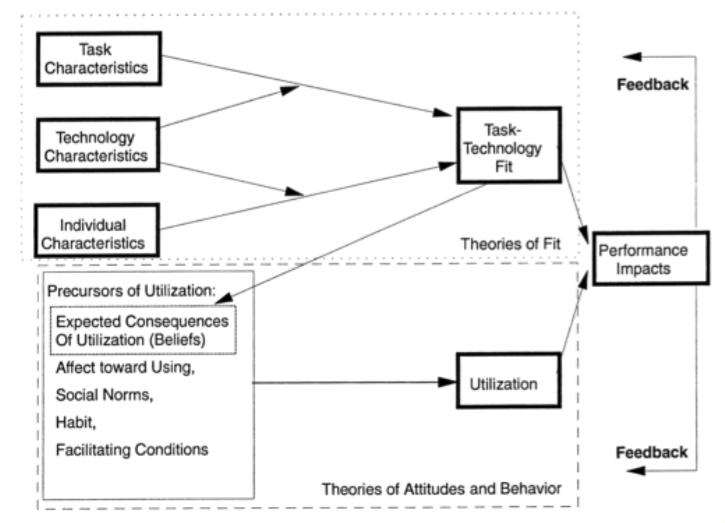
\includegraphics[width=\textwidth]{grafiken/ttf.png}
	\caption{Task-Technology Fit model\cite{MES10}}
\end{figure}

\subsection{Task characteristics}
\begin{itemize}
	\item Moving responsibility for test definition from developers to management staff
	\item Reduce time for bugs allocation and fixation
\end{itemize}


\subsection{Technology Characterisitcs}
\begin{itemize}
	\item Asynchronous software
	\item	Real-time software
\end{itemize}

\subsection{Individual Characterisitcs:}
\begin{itemize}
	\item  No developer background
\end{itemize}

\subsection{Task-Technology-Fit:}
\begin{itemize}
	\item Test Sheet is a representation for tests a developed with the goal to combine the power and completeness of formal programming language with a representation that is easy to understand and work with even for people with little IT knowledge\cite{ts}.
	\item node.js is an asynchronous event-driven framework designed to build scalable network applications.
	\item Optimization for real-time execution is done by changing test steps execution order and and position in the event loop with respect to their reference structure
	\item Automatization of bug reporting process directly to the developer (not covered in paper probably should not be mentioned)
\end{itemize}

\subsection{Utilization:}
\begin{itemize}
	\item Excel UX
	\item Simple conventions
\end{itemize}

\subsection{Performance Impact:}
\begin{itemize}
	\item Better / automated quality assurance process
	\item Wider spread of tasks and responsibility distributions amongst developers and managers
	\item Increased awareness / technical understanding of product functionality for managers 
	\item Time for training and using the test sheet required from managers
	\item Change of job descriptions / new tasks and responsibilities for managers
\end{itemize}

\section{Mistfits}
\paragraph{Functionality missfits} occur, when the way processes are executed using the ES leads to reduced efficiency and effectivenes compared to pre-ES outcomes 
\begin{itemize}
	\item No support for data validation by regular expressions
\end{itemize}

\paragraph{Data misfits}  occur, when data or data characteristics stored in or needed by the ES leads to data quality issues such as inaccuracy, inconsistent representation, inaccessibility, lack of timeliness or inappropriateness for users' context
\begin{itemize}
	\item none
\end{itemize}

\paragraph{Usability misfits}  occur, when the interactions with the ES required for task execution are cumbersome or confusing, i.e. requiring extra steps that add no value or introduce difficulty in entering or extracting information 
\begin{itemize}
	\item It is necessary to manually set define JSON object to be sent to API
	\item Test code should be stored on same machine as working system
\end{itemize}


\paragraph{Role misfits} occur, when the roles in the ES are inconcsistent with the skills available, create imbalances in the workload leading to bottlenecks and idle time, or generate mismatches between responsibility and authority 
\begin{itemize}
	\item Requires managements to store up-to-date code on their workstation
	\item Code generation requires call of command via CLI
\end{itemize}

\paragraph{Control misfits} occur, when the controls embedded in the ES provide too much control, inhibiting productivity, or too little control, leading to the inability to assess or monitor performance appropriately 
\begin{itemize}
		\item Requires managements to store up-to-date code on their workstation
		\item It is necessary to manually set define JSON object to be sent to API
\end{itemize}


\paragraph{Organizational culture misfits}  occur, when the ES requires ways of operating that countervene organizational norms 
\begin{itemize}
	\item Fact that test steps defined by non-developers staff confuses developers
\end{itemize}


\section{Benefits and affecting factors}
\paragraph{Organizational benefits} from system use from the perspective of senior management, is an overall measure of senior managemt's perception of the benefits from the IT-based application. Such benefits - which may be assessed either for the enterprise system investment overall, or from individual enterprise system projects - usually revolve around the software enabling faster, more accurate process coordination and execution, including links with business partners up and down the supply chain and greater accuracy of and visibility into organizational data, resulting in more tightly controlled organizational processes improved asset utilization and improved decision making.

\subsection{Short-term factor}
\paragraph{Functional Fit} is the extent to which the functional capabilities embedded and congigured within an enterprise system packge match the functionality that organization needs to operate effectively and efficiently. Saying that software has good functional fit is equivalent to saying that the processes supported by system are efficient and effiective for the organization and the software helps people in organization get their jobs done. It conceptualized as being delivered and measured project by project.
\paragraph{Oevercoming Organizational Inertia} is the extent to which members of the organization have been motivated to learn, use, and accept new system. During initial implementation and subsequent upgrade projects, considerable change-management effort, training, and support are needed to overcome organizational inertia.

\subsection{Long-term factor}
\paragraph{Integration} of information system is the unification of processes and/or data from multiple computer-based systems, not necessarily in the one organization.
\paragraph{Process optimization} is any attepmt to improve the efficiency and effectiveness of an organizations processes, ultimately in support of strategic goals.
\paragraph{Improved access to information} is any step take to increase the provision of timely, accurate, relevant information to key organizational decision making.
\paragraph{On-going major enterprise system improvement projects} is a measure of the number and extent of investment in major business improvement projects that an organization ha undertaken for improving and extending uts enterprise system. Major business projects are those that lead to changes in the way that work is done in the business.

\paragraph{Operational Benefits of Test Sheets Use}
\begin{itemize}
	\item Cycle time reduction
	\item Productivity improvement - Developers can concentrate more on creating and fixing code instead of running manual tests
	\item Quality improvement - Errors are identified earlier due to automated monitoring, bugs are easier identified before deployments
	\item Customer Service improvement - Less complaints from customers (!not descriptive "LESS")
\end{itemize}

\paragraph{Managerial:}
\begin{itemize}
	\item Resource management - No additional QA staff necessary
\end{itemize}

\paragraph{Organizational:}
\begin{itemize}
	\item Changing work patterns - Reduced workload on developers, increased product quality responsibility for managers
	\item Facilitating organizational learning - Managers learn / gain more technical understanding and feel empowered by owning the responsibility for the testing
\end{itemize}
%\begin{table}[h]
%	\begin{center}
%		\begin{tabular}{| l | l |  }
%			\hline
%			\textbf{Cost reduction} & +  \\
%			\hline
%			\textbf{Cycle time reduction} & + \\
%			\hline
%			\textbf{Productivity improvement} & +  \\
%			\hline
%			\textbf{Quality improvement} & + \\
%			\hline 
%			\textbf{Customer Service improvement} & + \\
%			\hline
%		\end{tabular}
%	\end{center}
%	\caption{Operational Benefits of Test Sheets Use}
%\end{table}
%
%\begin{table}[h]
%	\begin{center}
%		\begin{tabular}{| l | l |  }
%			\hline
%			\textbf{Resource management} & +  \\
%			\hline
%			\textbf{Decision making and planning} & + \\
%			\hline
%			\textbf{Performance} & +  \\
%			\hline
%		\end{tabular}
%	\end{center}
%	\caption{Managerial Benefits of Test Sheets Use}
%\end{table}
%
%\begin{table}[h]
%	\begin{center}
%		\begin{tabular}{| l | l |  }
%			\hline
%			\textbf{Business growth} & +  \\
%			\hline
%			\textbf{Business alliance} & + \\
%			\hline
%			\textbf{Building business innovations} & +  \\
%			\hline
%			\textbf{Building cost leadership} & + \\
%			\hline 
%			\textbf{Product differentiation} & + \\
%			\hline
%			\textbf{External linkages} & + \\
%			\hline
%		\end{tabular}
%	\end{center}
%	\caption{Strategic Benefits of Test Sheets Use}
%\end{table}
%
%\begin{table}[h]
%	\begin{center}
%		\begin{tabular}{| l | l |  }
%			\hline
%			\textbf{Business flexibility for future challenges} & +  \\
%			\hline
%			\textbf{IT cost reduction} & + \\
%			\hline
%			\textbf{IT infrastructure capabilities} & +  \\
%			\hline
%		\end{tabular}
%	\end{center}
%	\caption{IT infrastructure Benefits of Test Sheets Use}
%\end{table}
%
%\begin{table}[h]
%	\begin{center}
%		\begin{tabular}{| l | l |  }
%			\hline
%			\textbf{Changing work patterns} & +  \\
%			\hline
%			\textbf{Facilitating organizational learning} & + \\
%			\hline
%			\textbf{Empowerment} & +  \\
%			\hline
%			\textbf{Building common vision} & + \\
%			\hline
%		\end{tabular}
%	\end{center}
%	\caption{Organizational Benefits of Test Sheets Use}
%\end{table}


